\documentclass[11pt,a4paper]{article}
\usepackage[margin=21mm,headheight=16pt]{geometry}
\usepackage{fontspec}\setmainfont{Noto Serif}\setsansfont{Noto Sans}\setmonofont{Noto Sans Mono}
\usepackage{polyglossia}\setdefaultlanguage{turkish}
\usepackage{amsmath,amssymb,mathtools,graphicx,xcolor,booktabs,tabularx,array,enumitem}
\usepackage[most]{tcolorbox}\usepackage{fancyhdr,titlesec,needspace}
\usepackage[unicode,hidelinks,breaklinks]{hyperref}\usepackage{bookmark}
\definecolor{ink}{HTML}{18233A}\definecolor{accent}{HTML}{545AC4}\definecolor{green}{HTML}{087E66}\definecolor{paper}{HTML}{F3F5FA}
\color{ink}\setlength{\parindent}{0pt}\setlength{\parskip}{7pt}\linespread{1.10}
\setlength{\emergencystretch}{3em}\allowdisplaybreaks
\setlist{topsep=4pt,itemsep=4pt,leftmargin=*}
\pagestyle{fancy}\fancyhf{}\fancyhead[L]{\sffamily\small MÜHENDİSLİK MATEMATİĞİ}\fancyhead[R]{\sffamily\small Ders çalışma notları}\fancyfoot[L]{\sffamily\scriptsize Fotoğraflar + müfredat | 8 Kasım 2026}\fancyfoot[R]{\sffamily\thepage}
\titleformat{\section}{\Large\sffamily\bfseries\color{accent}}{\thesection}{.6em}{}
\titleformat{\subsection}{\large\sffamily\bfseries}{\thesubsection}{.6em}{}
\tcbset{enhanced,breakable,boxrule=.4pt,arc=2mm,left=3mm,right=3mm,top=2mm,bottom=2mm,before skip=8pt,after skip=8pt,fonttitle=\sffamily\bfseries,colback=paper,colframe=accent,coltitle=white}
\newcommand{\notebox}[2]{\begin{tcolorbox}[title={#1},colframe=accent!70!black]#2\end{tcolorbox}}
\hypersetup{pdfauthor={Mühendislik Matematiği Çalışma Atölyesi},pdfsubject={Ders fotoğrafları ve altı başlıklı müfredata göre özgün Türkçe çalışma notları}}
\begin{document}

\hypersetup{pdftitle={Doğrular, düzlemler ve kuadratik yüzeyler}}
{\sffamily\small\color{accent} ÇALIŞMA ATÖLYESİ / KONU 02\par}
\vspace{8mm}
{\Huge\sffamily\bfseries\raggedright\hyphenpenalty=10000 Doğrular, düzlemler ve kuadratik yüzeyler\par}
\vspace{3mm}
{\large Parametrik denklemler, açılar, uzaklıklar; küre, silindir, koni ve temel kuadriklerin kesitleri.\par}
\vspace{4mm}\hrule\vspace{4mm}\subsection*{Bu bölümün hedefleri}\begin{itemize}
\item Bir doğruyu nokta ve yönle, bir düzlemi nokta ve normalle kurmak.
\item Kesişim, açı ve uzaklıkta uygun vektörü belirlemek.
\item Kuadratik yüzeyleri işaretleri ve düzlem kesitleriyle tanımak.\end{itemize}
{\small\tableofcontents}\clearpage
\section{Uzayda doğru: nokta ve yön}
Bir doğrunun tek bir başlangıç noktası \(P_0\) ve sıfır olmayan bir doğrultu vektörü \(\mathbf u\) bilinirse tüm noktaları bir parametreyle üretilir. İki nokta verilmişse yön olarak aralarındaki fark alınır. Aynı doğru için başlangıç noktası veya yönün sıfır olmayan katı değişebilir.


{\small\[
\mathbf r(t)=\mathbf r_0+t\mathbf u,\quad x=x_0+at,\ y=y_0+bt,\ z=z_0+ct,\qquad t\in\mathbb R.
\]}
\(a,b,c\) sıfır değilse \((x-x_0)/a=(y-y_0)/b=(z-z_0)/c\) simetrik biçimi elde edilir. Bir bileşen sıfırsa ona ait koordinat sabittir. Örneğin \(b=0\) ise \(y=y_0\) ayrıca yazılır; sıfıra bölme yapılmaz.

\Needspace{10\baselineskip}\begin{tcolorbox}[title={Örnek 2.1 | İki noktadan geçen doğru},colframe=accent]\(A=(0,1,2)\), \(B=(3,1,-1)\) doğrusunu bulunuz.
\par\vspace{1mm}{\scriptsize\sffamily Ders fotoğrafından | \nolinkurl{IMG-20261009-WA0032.jpg}}\end{tcolorbox}
\begin{tcolorbox}[title={Adım adım çözüm},colback=green!3!white,colframe=green]\begin{enumerate}
\item \(\overrightarrow{AB}=(3,0,-3)\), bunun yerine \((1,0,-1)\) kullanılabilir.
\item \(x=t,\ y=1,\ z=2-t\). Kartezyen biçim \(x=2-z,\ y=1\). Parametre 0 iken A, 3 iken B elde edilir.
\end{enumerate}\end{tcolorbox}
\Needspace{10\baselineskip}\begin{tcolorbox}[title={Örnek 2.2 | Nokta ve paralel vektör},colframe=accent]\(A=(1,2,3)\) noktasından geçen ve \((2,3,0)\) yönüne paralel doğruyu yazınız.
\par\vspace{1mm}{\scriptsize\sffamily Ders fotoğrafından | \nolinkurl{IMG-20261009-WA0030.jpg}}\end{tcolorbox}
\begin{tcolorbox}[title={Adım adım çözüm},colback=green!3!white,colframe=green]\begin{enumerate}
\item \(x=1+2t,\ y=2+3t,\ z=3\).
\item Simetrik gösterim \((x-1)/2=(y-2)/3\), ayrıca \(z=3\). İki denklem uzayda tek doğruyu belirler.
\end{enumerate}\end{tcolorbox}
\section{Doğruların konumları ve açıları}
İki doğru karşılaştırılırken ilk adım yön vektörlerini karşılaştırmaktır. Paralel yönler için bir doğrunun noktası ötekinin üzerinde de bulunuyorsa doğrular çakışıktır. Paralel olmayan yönlerde kesişim için iki parametreli üç denklem çözülür. Çözüm yoksa doğrular aykırıdır.


{\small\[
\cos\varphi=\frac{|\mathbf u\cdot\mathbf v|}{\|\mathbf u\|\|\mathbf v\|},\qquad 0\le\varphi\le\frac\pi2.
\]}
\notebox{Uzayda diklik nüansı}{\(\mathbf u\cdot\mathbf v=0\) yönlerin dik olduğunu söyler. Doğruların dik kesiştiğini söylemek için ayrıca kesiştiklerini kontrol et; uzayda aykırı doğruların da yönleri dik olabilir.}
\Needspace{10\baselineskip}\begin{tcolorbox}[title={Örnek 2.3 | Tahtadaki sıfır paydalı gösterim},colframe=accent]Tahtada \(x/1=y/1=z/0\) ve \((x-1)/1=y/(-1)=z/0\) ile belirtilen doğruların açısı nedir?
\par\vspace{1mm}{\scriptsize\sffamily Ders fotoğrafından | \nolinkurl{IMG-20261001-WA0014.jpg}}\end{tcolorbox}
\begin{tcolorbox}[title={Adım adım çözüm},colback=green!3!white,colframe=green]\begin{enumerate}
\item Bu gösterimde \(z/0\) gerçek bir bölüm değildir; \(z=0\) kısıtının kısa yazımı olarak yorumlanır. Parametrik biçimler \((t,t,0)\) ve \((1+s,-s,0)\) olur.
\item Yönler \((1,1,0)\), \((1,-1,0)\), çarpımları 0. \(t=1+s=-s\) den \(t=1/2,s=-1/2\); kesişim \((1/2,1/2,0)\). Dolayısıyla açı \(90^\circ\).
\end{enumerate}\end{tcolorbox}
\section{Düzlem denklemi ve normal vektör}
Bir düzlemin içinde pek çok doğrultu vardır; bunların tümüne dik olan bir normal vektör düzlemin yönelimini belirler. \(P_0\) düzlem üzerinde ve \(\mathbf n=(A,B,C)\ne\mathbf0\) normal ise her \(P\) noktası için \(\overrightarrow{P_0P}\cdot\mathbf n=0\) yazılır.


{\small\[
A(x-x_0)+B(y-y_0)+C(z-z_0)=0\quad\Longleftrightarrow\quad Ax+By+Cz+D=0.
\]}
Üç nokta verildiğinde aynı başlangıçtan çıkan iki fark vektörünün vektörel çarpımı normal olur. Çarpım sıfırsa noktalar doğrudaştır ve tek bir düzlem belirlemez. Bulunan denklemi her üç noktada denemek iyi bir hata kontrolüdür.

\Needspace{10\baselineskip}\begin{tcolorbox}[title={Örnek 2.4 | Koordinat eksenlerini kesen düzlem},colframe=accent]\(A=(1,0,0),B=(0,1,0),C=(0,0,1)\) noktalarından geçen düzlemi bulunuz.
\par\vspace{1mm}{\scriptsize\sffamily Ders fotoğrafından | \nolinkurl{IMG-20261001-WA0014.jpg}}\end{tcolorbox}
\begin{tcolorbox}[title={Adım adım çözüm},colback=green!3!white,colframe=green]\begin{enumerate}
\item \(\overrightarrow{AB}=(-1,1,0)\), \(\overrightarrow{AC}=(-1,0,1)\). Çarpımları \((1,1,1)\).
\item \((x-1)+y+z=0\), yani \(x+y+z=1\). Üç nokta da denklemi sağlar.
\end{enumerate}\end{tcolorbox}
\Needspace{10\baselineskip}\begin{tcolorbox}[title={Örnek 2.5 | Nokta ve normal ile düzlem},colframe=accent]\(A=(2,3,4)\) noktasından geçen, normali \((1,3,4)\) olan düzlemi bulunuz.
\par\vspace{1mm}{\scriptsize\sffamily Ders fotoğrafından | \nolinkurl{IMG-20261023-WA0030.jpg}}\end{tcolorbox}
\begin{tcolorbox}[title={Adım adım çözüm},colback=green!3!white,colframe=green]\begin{enumerate}
\item \((x-2)+3(y-3)+4(z-4)=0\).
\item Düzenlenince \(x+3y+4z-27=0\). Normalin herhangi bir sıfır olmayan katı aynı düzlemi verir.
\end{enumerate}\end{tcolorbox}
\section{Doğru-düzlem ve iki düzlemin kesişimi}
Doğruyu düzlemde yerine koyunca parametre için tek bir lineer denklem çıkar. \(\mathbf n\cdot\mathbf u\ne0\) ise tek kesişim vardır. \(\mathbf n\cdot\mathbf u=0\) ise doğru düzleme paraleldir; başlangıç noktası denklemi sağlıyorsa doğru düzlemin içindedir.

\Needspace{10\baselineskip}\begin{tcolorbox}[title={Örnek 2.6 | Dersteki doğru-düzlem kesişimi},colframe=accent]\((x-2)/1=y/2=(z+1)/(-1)\) doğrusu ile \(x-y+2z=3\) düzleminin kesişimi nedir?
\par\vspace{1mm}{\scriptsize\sffamily Ders fotoğrafından | \nolinkurl{IMG-20261001-WA0014.jpg}}\end{tcolorbox}
\begin{tcolorbox}[title={Adım adım çözüm},colback=green!3!white,colframe=green]\begin{enumerate}
\item \(x=2+t,\ y=2t,\ z=-1-t\) yazılır.
\item Yerine koyunca \((2+t)-2t+2(-1-t)=3\), yani \(-3t=3\). \(t=-1\) ile nokta \((1,-2,0)\). Kontrol: \(1-(-2)+0=3\).
\end{enumerate}\end{tcolorbox}
Paralel olmayan iki düzlemin kesişim doğrusunun yönü \(\mathbf n_1\times\mathbf n_2\) olur. Bir koordinatı uygun seçip kalan iki denklemi çözerek doğru üzerinde bir nokta bulunur. İki normal paralelse kesişim bir doğru olamaz; düzlemler çakışık veya ayrık paraleldir.

\Needspace{10\baselineskip}\begin{tcolorbox}[title={Örnek 2.7 | İki düzlemin arakesiti},colframe=accent]\(x+y+z=2\) ve \(x-y+z=0\) düzlemlerinin kesişimini yazınız.
\par\vspace{1mm}{\scriptsize\sffamily Pekiştirme}\end{tcolorbox}
\begin{tcolorbox}[title={Adım adım çözüm},colback=green!3!white,colframe=green]\begin{enumerate}
\item Denklemleri çıkarınca \(2y=2\), yani \(y=1\). Sonra \(x+z=1\).
\item \(x=t\) seçilirse \(\mathbf r(t)=(t,1,1-t)\). Yön \((1,0,-1)\), normallerin vektörel çarpımına paraleldir.
\end{enumerate}\end{tcolorbox}
\section{Açı sorularında hangi vektör kullanılır?}
\begin{center}\small\renewcommand{\arraystretch}{1.35}\begin{tabularx}{\linewidth}{>{\raggedright\arraybackslash}X >{\raggedright\arraybackslash}X >{\raggedright\arraybackslash}X}\toprule
\textbf{Geometrik çift} & \textbf{İlişkilendirilecek vektör} & \textbf{Formül}\\\midrule
Doğru - doğru & İki yön & \(\cos\varphi=|\mathbf u\cdot\mathbf v|/(\|\mathbf u\|\|\mathbf v\|)\)\\
Düzlem - düzlem & İki normal & \(\cos\varphi=|\mathbf n_1\cdot\mathbf n_2|/(\|\mathbf n_1\|\|\mathbf n_2\|)\)\\
Doğru - düzlem & Yön ve normal & \(\sin\varphi=|\mathbf u\cdot\mathbf n|/(\|\mathbf u\|\|\mathbf n\|)\)\\
\bottomrule\end{tabularx}\end{center}
Doğru ile düzlem açısında sinüs kullanılmasının nedeni, yönle normal arasındaki dar açıya tümleyen olmasıdır. Doğru düzleme paralelse \(\mathbf u\cdot\mathbf n=0\) ve açı 0; düzleme dikse \(\mathbf u\parallel\mathbf n\) ve açı \(90^\circ\) çıkar. İki düzlemin dikliği normal vektörlerin dikliğidir.

\section{Noktanın doğruya ve düzleme uzaklığı}
Uzaklık her zaman en kısa, dolayısıyla dik bağlantının uzunluğudur. Nokta-doğru uzaklığında \(\overrightarrow{AP}\) ile yön vektörünün oluşturduğu paralelkenarın alanı tabana bölünür. Nokta-düzlem uzaklığında ise \(\overrightarrow{P_0P}\) normal doğrultusuna izdüşürülür.


{\small\[
d(P,\ell)=\frac{\|\overrightarrow{AP}\times\mathbf u\|}{\|\mathbf u\|},\qquad d(P,\Pi)=\frac{|Ax_P+By_P+Cz_P+D|}{\sqrt{A^2+B^2+C^2}}.
\]}
\Needspace{10\baselineskip}\begin{tcolorbox}[title={Örnek 2.8 | Tahtadaki nokta-doğru uzaklığı},colframe=accent]\(P=(2,3,-1)\) noktasının \((x-1)/1=(y-2)/1=(z-13)/4\) doğrusuna uzaklığını bulunuz.
\par\vspace{1mm}{\scriptsize\sffamily Ders fotoğrafından | \nolinkurl{IMG-20261023-WA0057.jpg}}\end{tcolorbox}
\begin{tcolorbox}[title={Adım adım çözüm},colback=green!3!white,colframe=green]\begin{enumerate}
\item Doğru üzerinde \(A=(1,2,13)\), yön \(\mathbf u=(1,1,4)\). \(\overrightarrow{AP}=(1,1,-14)\).
\item \(\overrightarrow{AP}\times\mathbf u=(18,-18,0)\); normu \(18\sqrt2\). Yönün normu \(\sqrt{18}=3\sqrt2\). Uzaklık 6.
\end{enumerate}\end{tcolorbox}
\Needspace{10\baselineskip}\begin{tcolorbox}[title={Örnek 2.9 | Çalışma sorusu: nokta-düzlem uzaklığı},colframe=accent]\(P=(1,0,2)\) noktasının \(x+2y-2z+4=0\) düzlemine uzaklığı nedir?
\par\vspace{1mm}{\scriptsize\sffamily Ders fotoğrafından | \nolinkurl{IMG-20261001-WA0014.jpg}}\end{tcolorbox}
\begin{tcolorbox}[title={Adım adım çözüm},colback=green!3!white,colframe=green]\begin{enumerate}
\item Pay \(|1+0-4+4|=1\), payda \(\sqrt{1+4+4}=3\). Uzaklık \(1/3\).
\item Dik izdüşüm noktası \(H=P-\frac{1}{9}(1,2,-2)=(8/9,-2/9,20/9)\). Denkleme koyunca sıfır çıkar ve \(\|P-H\|=1/3\).
\end{enumerate}\end{tcolorbox}
Paralel düzlemler aynı normal katsayılarıyla yazılmışsa \(d=|D_2-D_1|/\|\mathbf n\|\). Katsayılar yalnızca orantılıysa önce aynı normale dönüştür. Aykırı doğrular için \(d=|(\mathbf r_2-\mathbf r_1)\cdot(\mathbf u\times\mathbf v)|/\|\mathbf u\times\mathbf v\|\); bu son bağıntı paralel doğrularda kullanılmaz.

\section{Küre ve kareye tamamlama}
Küre, bir merkezden eşit uzaklıktaki noktaların kümesidir. Genel denklemde üç kare teriminin katsayısı aynı ve çapraz terimler yoksa kareye tamamlama ile merkez ve yarıçap okunabilir. Sabit terimden yarıçapın karesini yanlış işaretle çıkarmamak için her koordinatı ayrı düzenle.


{\small\[
(x-a)^2+(y-b)^2+(z-c)^2=R^2.
\]}
\Needspace{10\baselineskip}\begin{tcolorbox}[title={Örnek 2.10 | Dersteki küre sorusu},colframe=accent]\(x^2+y^2+z^2+4x-6y+2z-11=0\) küresinin merkezi ve yarıçapı nedir?
\par\vspace{1mm}{\scriptsize\sffamily Ders fotoğrafından | \nolinkurl{IMG-20261009-WA0032.jpg}}\end{tcolorbox}
\begin{tcolorbox}[title={Adım adım çözüm},colback=green!3!white,colframe=green]\begin{enumerate}
\item \((x+2)^2-4+(y-3)^2-9+(z+1)^2-1-11=0\).
\item \((x+2)^2+(y-3)^2+(z+1)^2=25\). Merkez \((-2,3,-1)\), yarıçap 5.
\end{enumerate}\end{tcolorbox}
\section{Silindirler ve kuadratik yüzeyleri tanıma}
Bir denklemde bir koordinat hiç görünmüyorsa düzlemdeki eğri o koordinat boyunca taşınır. Örneğin \(x^2+y^2=4\), \(z\) eksenine paralel dairesel silindirdir; \(z=y^2\), \(x\) doğrultusunda uzayan parabolik silindirdir. Silindirin mutlaka dairesel olması gerekmez.

\begin{center}\small\renewcommand{\arraystretch}{1.35}\begin{tabularx}{\linewidth}{>{\raggedright\arraybackslash}X >{\raggedright\arraybackslash}X >{\raggedright\arraybackslash}X}\toprule
\textbf{Yüzey} & \textbf{Standart örnek} & \textbf{Ayırt edici özellik}\\\midrule
Elipsoid & \(x^2/a^2+y^2/b^2+z^2/c^2=1\) & Üç kare de pozitif; kapalı.\\
Tek kanatlı hiperboloid & \(x^2/a^2+y^2/b^2-z^2/c^2=1\) & Bir eksi; eksi işaretli eksen boyunca tek parça.\\
Çift kanatlı hiperboloid & \(-x^2/a^2-y^2/b^2+z^2/c^2=1\) & İki eksi; artı işaretli eksende iki parça.\\
Eliptik koni & \(z^2/c^2=x^2/a^2+y^2/b^2\) & Sıfır seviyesi; iki kanat tepe noktasında birleşir.\\
Eliptik paraboloid & \(z=x^2/a^2+y^2/b^2\) & Yatay kesit elips; dikey kesit parabol.\\
Hiperbolik paraboloid & \(z=x^2/a^2-y^2/b^2\) & Eyer; iki ana doğrultuda ters bükülme.\\
\bottomrule\end{tabularx}\end{center}
\begin{center}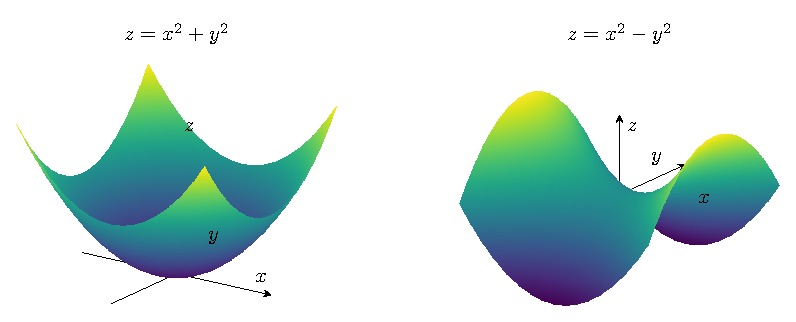
\includegraphics[width=.94\linewidth,height=65mm,keepaspectratio]{../assets/figures/quadrics.pdf}\par{\small\sffamily Eliptik paraboloid ve hiperbolik paraboloid: kesitlerin işareti yüzeyin biçimini belirler.}\end{center}
\notebox{Eksenleri ezberleme}{Önce denklemi standart biçime getir. Eksi işaretli ya da tek başına kalan değişken değişirse yüzeyin ekseni de değişir; yüzey adını yalnızca \(z\) eksenine bakarak seçme.}
\Needspace{14\baselineskip}\section{Fotoğraflardan ek analitik geometri çözümleri}
\Needspace{10\baselineskip}\begin{tcolorbox}[title={Örnek 2.11 | Doğruya dik düzlem},colframe=accent]P=(2,3,5) noktasından geçen, \((x-1)/4=(y-2)/(-1)=(z+1)/6\) doğrusuna dik düzlemi bulunuz.
\par\vspace{1mm}{\scriptsize\sffamily Ders fotoğrafından | \nolinkurl{IMG-20261002-WA0024.jpg}}\end{tcolorbox}
\begin{tcolorbox}[title={Adım adım çözüm},colback=green!3!white,colframe=green]\begin{enumerate}
\item Doğrunun yönü \((4,-1,6)\), istenen düzlemin normalidir. \(4(x-2)-(y-3)+6(z-5)=0\).
\item Denklem \(4x-y+6z-35=0\). P yi yerine koyunca sıfır, doğru yönüyle normalin paralelliği ise dikliği doğrular.
\end{enumerate}\end{tcolorbox}
\Needspace{10\baselineskip}\begin{tcolorbox}[title={Örnek 2.12 | Aynı yöntemin ikinci örneği},colframe=accent]A=(2,3,-5) noktasından geçen, normali (7,3,4) olan düzlemi yazınız.
\par\vspace{1mm}{\scriptsize\sffamily Ders fotoğrafından | \nolinkurl{IMG-20261002-WA0020.jpg}}\end{tcolorbox}
\begin{tcolorbox}[title={Adım adım çözüm},colback=green!3!white,colframe=green]\begin{enumerate}
\item \(7(x-2)+3(y-3)+4(z+5)=0\).
\item Sonuç \(7x+3y+4z-3=0\). Üçüncü koordinat -5 olduğu için parantezde z+5 gelir.
\end{enumerate}\end{tcolorbox}
\Needspace{10\baselineskip}\begin{tcolorbox}[title={Örnek 2.13 | Tahtadaki ikinci kesişim örneği},colframe=accent]\((x-1)/2=(y-1)/(-1)=z/3\) doğrusu ile \(2x+3y+z+11=0\) düzleminin kesişimi nedir?
\par\vspace{1mm}{\scriptsize\sffamily Ders fotoğrafından | \nolinkurl{IMG-20261002-WA0026.jpg}}\end{tcolorbox}
\begin{tcolorbox}[title={Adım adım çözüm},colback=green!3!white,colframe=green]\begin{enumerate}
\item \(x=1+2t,y=1-t,z=3t\). Yerine koyunca \(2+4t+3-3t+3t+11=0\), yani \(4t+16=0\).
\item t=-4, kesişim \((-7,5,-12)\). Kontrol \(-14+15-12+11=0\).
\end{enumerate}\end{tcolorbox}
\Needspace{10\baselineskip}\begin{tcolorbox}[title={Örnek 2.14 | İki düzlemin arakesiti: tahta örneği},colframe=accent]\(x+y+z=3\) ve \(x-y+z=1\) düzlemlerinin arakesitini bulunuz.
\par\vspace{1mm}{\scriptsize\sffamily Ders fotoğrafından | \nolinkurl{IMG-20261002-WA0026.jpg}}\end{tcolorbox}
\begin{tcolorbox}[title={Adım adım çözüm},colback=green!3!white,colframe=green]\begin{enumerate}
\item Çıkarınca y=1. z=0 seçilirse x=2; nokta (2,1,0). Normal çarpımı (2,0,-2), eşdeğer yön (1,0,-1).
\item Doğru \((x,y,z)=(2,1,0)+t(1,0,-1)\). Her iki düzlem denklemine de tüm t ler için uyar.
\end{enumerate}\end{tcolorbox}
\Needspace{10\baselineskip}\begin{tcolorbox}[title={Örnek 2.15 | Defterdeki ikinci küre},colframe=accent]\(x^2+y^2+z^2-2x-4y-6z-2=0\) küresinin merkezi ve yarıçapını bulunuz.
\par\vspace{1mm}{\scriptsize\sffamily Ders fotoğrafından | \nolinkurl{IMG-20261009-WA0028.jpg}}\end{tcolorbox}
\begin{tcolorbox}[title={Adım adım çözüm},colback=green!3!white,colframe=green]\begin{enumerate}
\item \((x-1)^2+(y-2)^2+(z-3)^2=16\).
\item Merkez (1,2,3), yarıçap 4. Tam kareler açıldığında sabit 14, sağdan taşınan 16 ile -2 elde edilmesi kontrol sağlar.
\end{enumerate}\end{tcolorbox}
\section{Kesitlerle çizim: adım adım}
\begin{enumerate}
\item Ötelemeler varsa \(X=x-a,Y=y-b,Z=z-c\) ile merkezi veya tepeyi belirle.
\item \(x=0,y=0,z=0\) kesitlerini al; elips, hiperbol veya parabol olup olmadığını incele.
\item \(z=k\) gibi paralel kesitlerde boyutun nasıl değiştiğini bul.
\item Simetriyi, eksen kesişimlerini ve varsa boş kesitleri işaretle.
\end{enumerate}
\Needspace{10\baselineskip}\begin{tcolorbox}[title={Örnek 2.16 | İki yüzeyin kesitlerini karşılaştır},colframe=accent]\(x^2+y^2-z^2=1\) ve \(z^2-x^2-y^2=1\) neden farklıdır?
\par\vspace{1mm}{\scriptsize\sffamily Pekiştirme}\end{tcolorbox}
\begin{tcolorbox}[title={Adım adım çözüm},colback=green!3!white,colframe=green]\begin{enumerate}
\item İlkinde \(z=k\) için \(x^2+y^2=1+k^2\). Her k için çember vardır; en dar kesit \(z=0\) düzlemindedir. Tek kanatlı hiperboloid.
\item İkincide \(x^2+y^2=k^2-1\). \(|k|<1\) için kesit yok; \(k=\pm1\) için bir nokta, dışarıda çember vardır. Çift kanatlı hiperboloid.
\end{enumerate}\end{tcolorbox}
\Needspace{10\baselineskip}\begin{tcolorbox}[title={Örnek 2.17 | Pekiştirme: yüzeyi tanı},colframe=accent]\(z=4-x^2-y^2\) yüzeyinin tepesini, açılma yönünü ve \(z=0\) kesitini bulunuz.
\par\vspace{1mm}{\scriptsize\sffamily Pekiştirme}\end{tcolorbox}
\begin{tcolorbox}[title={Adım adım çözüm},colback=green!3!white,colframe=green]\begin{enumerate}
\item Tepe \((0,0,4)\), karelerin katsayıları negatif olduğundan aşağı açılan eliptik paraboloid.
\item \(z=0\) kesiti \(x^2+y^2=4\), yarıçapı 2 olan çember. \(z>4\) için kesit yoktur.
\end{enumerate}\end{tcolorbox}

\clearpage
\section*{Kaynaklar ve kapsam}
\addcontentsline{toc}{section}{Kaynaklar ve kapsam}
Bu metin 156 ders/defter fotoğrafı ve altı başlıklı müfredata göre özgün olarak yazıldı. Fotoğraflar dersin sıra ve örneklerini belirler. Ek sorular pekiştirme olarak etiketlidir; çıkmış sınav sorusu iddiası yoktur. Soluk semboller tahminle aktarılmadı. Gradyan ve yönlü türev, müfredat gereği tamamlanan anlatımdır. Fotoğraf bazında inceleme dizini web sitesinde ve analysis/FOTOGRAF\_INCELEMESI.md dosyasında bulunur.
\textbf{Birincil ders malzemesi}. Kullanıcının sağladığı 156 JPG ders/defter fotoğrafı ve mufredat.png. Dosya tarihleri ders tarihi olarak varsayılmadı. Konu-fotoğraf eşleştirmesi fotoğraf dizinindedir.\par
\textbf{Erwin Kreyszig · Advanced Engineering Mathematics}. Dersin belirtilen kitabı. Wiley 10. baskı bölüm diziniyle vektör diferansiyel hesabı başlığı eşleştirildi; tam kitap dosyası sağlanmadı. Kitaptan birebir metin veya soru aktarımı yapılmadı.
{\footnotesize\url{https://bcs.wiley.com/he-bcs/Books?action=contents&bcsId=6140&itemId=0470458364}}\par
\textbf{KOCW · Kreyszig temelli Bölüm 9 ders notları}. Sungkyunkwan / Kim Munhyeon, vektörler ve vektör fonksiyonları. Açık üniversite notu kavram ve formül kontrolünde kullanıldı. Buradaki Türkçe açıklamalar ve çözümler özgün olarak yazıldı.
{\footnotesize\url{https://contents.kocw.net/KOCW/document/2015/sungkyunkwan/kimmunhyeon3/8.pdf}}\par
\textbf{Zill ve Wright · Calculus / Matematik}. Kullanıcının verdiği bibliyografya: İ. N. Cangül çevirisi, Nobel, 2013. Tam metne erişilmedi; baskıya özgü sayfa ve soru numarası atfedilmedi.\par
\textbf{Mustafa Balcı · Genel Matematik II}. Kullanıcının verdiği bibliyografya: Sürat, 2013. Tam metin sağlanmadı; bu kitaptan doğrulanmış alıntı veya sayfa atfı yapılmadı.\par
\textbf{MIT OCW · 18.02 ders notları}. Denis Auroux, 2007. Ders düzeni ve kavram denetimi için açık ders dizini. Müfredat dışındaki çok katlı integraller ve integral teoremleri bu çalışmaya eklenmedi.
{\footnotesize\url{https://ocw.mit.edu/courses/18-02-multivariable-calculus-fall-2007/pages/lecture-notes/}}\par
\textbf{MIT · Teğet düzlem ve gradyan}. Gradyanın teğet düzlem ve yönlü türevle ilişkisi için açık teknik kontrol kaynağı. Konuya eklenen örnekler özgün pekiştirme sorularıdır.
{\footnotesize\url{https://www.ocw.mit.edu/ans7870/18/18.013a/textbook/HTML/chapter06/section05.html}}\par
\end{document}
